\documentclass[
	12pt,
	BCOR=5mm,
	DIV=12,
	headinclude=on,
	footinclude=off,
	parskip=half,
	bibliography=totoc,
	listof=entryprefix,
	toc=listof,
	numbers=noenddot,
	plainfootsepline
]{scrreprt}

%	Konfigurationsdatei einziehen
% !TEX root =  master.tex

%		LANGUAGE SETTINGS AND FONT ENCODING 
%
\usepackage[ngerman]{babel} 	% German language
\usepackage[utf8]{inputenc}
\usepackage[german=quotes]{csquotes} 	% correct quotes using \enquote{}
\usepackage[T1]{fontenc}


%\usepackage[english]{babel}   % For english language
%\usepackage{csquotes} 	% Richtiges Setzen der Anführungszeichen mit \enquote{}

% 		HYPERREF
%
\usepackage[
	hidelinks=true % keine roten Markierungen bei Links
]{hyperref}

% Zwei eigene Befehle zum Setzen von Autor und Titel. Ausserdem werden die PDF-Informationen richtig gesetzt.
\newcommand{\TitelDerArbeit}[1]{\def\DerTitelDerArbeit{#1}\hypersetup{pdftitle={#1}}}
\newcommand{\AutorDerArbeit}[1]{\def\DerAutorDerArbeit{#1}\hypersetup{pdfauthor={#1}}}
\newcommand{\Firma}[1]{\def\DerNameDerFirma{#1}}
\newcommand{\Kurs}[1]{\def\DieKursbezeichnung{#1}}


% Correct superscripts 
\usepackage{fnpct}




%		CALCULATIONS
%
\usepackage{calc} % Used for extra space below footsepline



%		BIBLIOGRAPHY SETTINGS
%

% Uncomment the next three lines for author-year-style with footnotes (Chicago)
\usepackage[backend=biber, autocite=footnote, style=authoryear, dashed=false]{biblatex} 	%Use Author-Year-Cites with footnotes
\AdaptNoteOpt\footcite\multfootcite   %will add  separators if footcite is called multiple consecutive times 
\AdaptNoteOpt\autocite\multautocite % will add  separators if autocite is called multiple consecutive times

% Uncomment the next line for IEEE-style 
% \usepackage[backend=biber, autocite=inline, style=ieee]{biblatex} 	% Use IEEE-Style (e.g. [1])

% Uncomment the next line for alphabetic style 
% \usepackage[backend=biber, autocite=inline, style=alphabetic]{biblatex} 	% Use alphabetic style (e.g. [TGK12])

% Uncomment the next two lines vor Harvard-Style 
%\usepackage[backend=biber, style=apa]{biblatex} 	
%\DeclareLanguageMapping{german}{german-apa}


\DefineBibliographyStrings{ngerman}{  %Change u.a. to et al. (german only!)
	andothers = {{et\,al\adddot}},
}

%%% Uncomment the following lines to support hard URL breaks in bibliography 
%\apptocmd{\UrlBreaks}{\do\f\do\m}{}{}
%\setcounter{biburllcpenalty}{9000}% Kleinbuchstaben
%\setcounter{biburlucpenalty}{9000}% Großbuchstaben


\setlength{\bibparsep}{\parskip}		%add some space between biblatex entries in the bibliography
\addbibresource{bibliography.bib}	%Add file bibliography.bib as biblatex resource


%		FOOTNOTES 
%
% Count footnotes over chapters
\usepackage{chngcntr}
\counterwithout{footnote}{chapter}

%	ACRONYMS
%%%
%%% WICHTIG: Installieren Sie das neueste Acronyms-Paket!!!
%%%
\makeatletter
\usepackage[printonlyused]{acronym}
\@ifpackagelater{acronym}{2015/03/20}
  {%
    \renewcommand*{\aclabelfont}[1]{\textbf{\textsf{\acsfont{#1}}}}
  }%
  {%
  }%
\makeatother

%		LISTINGS
\usepackage{listings}	%Format Listings properly
\renewcommand{\lstlistingname}{Quelltext} 
\renewcommand{\lstlistlistingname}{Quelltextverzeichnis}
\lstset{numbers=left,
	numberstyle=\tiny,
	captionpos=b,
	basicstyle=\ttfamily\small}


%		EXTRA PACKAGES
\usepackage{lipsum}    %Blindtext
\usepackage{graphicx} % use various graphics formats
\usepackage[german]{varioref} 	% nicer references \vref
\usepackage{caption}	%better Captions
\usepackage{booktabs} %nicer Tabs
\usepackage{array}
%\newcolumntype{P}[1]{>{\raggedright\arraybackslash}p{#1}}


%		ALGORITHMS
\usepackage{algorithm}
\usepackage{algpseudocode}
\renewcommand{\listalgorithmname}{Algorithmenverzeichnis }
\floatname{algorithm}{Algorithmus}


%		FONT SELECTION: Entweder Latin Modern oder Times / Helvetica
\usepackage{lmodern} %Latin modern font
%\usepackage{mathptmx}  %Helvetica / Times New Roman fonts (2 lines)
%\usepackage[scaled=.92]{helvet} %Helvetica / Times New Roman fonts (2 lines)

%		PAGE HEADER / FOOTER
%	    Warning: There are some redefinitions throughout the master.tex-file!  DON'T CHANGE THESE REDEFINITIONS!
\RequirePackage[automark,headsepline,footsepline]{scrpage2}
\pagestyle{scrheadings}
\renewcommand*{\pnumfont}{\upshape\sffamily}
\renewcommand*{\headfont}{\upshape\sffamily}
\renewcommand*{\footfont}{\upshape\sffamily}
\renewcommand{\chaptermarkformat}{}
\RedeclareSectionCommand[beforeskip=0pt]{chapter}
\clearscrheadfoot

\ifoot[\rule{0pt}{\ht\strutbox+\dp\strutbox}DHBW Mannheim]{\rule{0pt}{\ht\strutbox+\dp\strutbox}DHBW Mannheim}
\ofoot[\rule{0pt}{\ht\strutbox+\dp\strutbox}\pagemark]{\rule{0pt}{\ht\strutbox+\dp\strutbox}\pagemark}

\ohead{\headmark}


\begin{document}

\TitelDerArbeit{TODO}
\AutorDerArbeit{Aaron Schweig}
\Firma{Hays AG}
\Kurs{WWI18SEC}

\begin{titlepage}
\begin{minipage}{\textwidth}
		\vspace{-2cm}
		\noindent 
		% \includegraphics[scale=0.71]{img/firmenlogo.jpg} 
		\hfill   
\includegraphics{img/logo.jpg}
\end{minipage}
\vspace{1em}
\sffamily
\begin{center}
	\textsf{\large{}Duale Hochschule Baden-W\"urttemberg\\[1.5mm] Mannheim}\\[2em]
	\textsf{\textbf{\Large{}Projektarbeit 2}}\\[3mm]
	\textsf{\textbf{\DerTitelDerArbeit}} \\[1.5cm]
	\textsf{\textbf{\Large{}Studiengang Wirtschaftsinformatik}\\[3mm] \textsf{Studienrichtung Software Engineering}}
	
	\vspace{3em}
	% \textsf{\Large{Sperrvermerk}}
\vfill

\begin{minipage}{\textwidth}

\begin{tabbing}
	Wissenschaftlicher Betreuer: \hspace{0.85cm}\=\kill
	Verfasser/in: \> \DerAutorDerArbeit \\[1.5mm]
	Matrikelnummer: \> 6161622 \\[1.5mm]
	Firma: \> \DerNameDerFirma  \\[1.5mm]
	Abteilung: \> Softwareentwicklung \\[1.5mm]
	Kurs: \> \DieKursbezeichnung \\[1.5mm]
	Studiengangsleiter: \> Prof. Dr. Sebastian Ritterbusch  \\[1.5mm]
	Wissenschaftlicher Betreuer: \> Prof. Dr. Julian Reichwald \\
	\> j.reichwald@hs-mannheim.de \\
	% \> +49 151 / 123 456 \\[1.5mm]
	Firmenbetreuer: \> Philip Liening \\
	\> philip.liening@hays.de \\
	% \> +49 151 / 123 456 \\[1.5mm]
	Bearbeitungszeitraum: \> 18.05.2020 -- 01.09.2020
\end{tabbing}
\end{minipage}

\end{center}

\end{titlepage}

\pagenumbering{roman} % Römische Seitennummerierung
\normalfont

%	Kurzfassung
\chapter*{Kurzfassung}
\begingroup
\begin{table}[h!]
\setlength\tabcolsep{0pt}
\begin{tabular}{p{3.7cm}p{11.7cm}}
Titel: & \DerTitelDerArbeit \\
Verfasser/in: & \DerAutorDerArbeit \\
Kurs: & \DieKursbezeichnung \\
Ausbildungsstätte: & \DerNameDerFirma\\
\end{tabular}
\end{table}
\endgroup

Folgende Arbeit beschreibt ein Konzept für eine graphbasierte Service-Registry. Dabei wurde eine Gegenüberstellung zwischen dem hergeleiteten Konzept der Service-Registry und einer Komposition verschiedener Produkte zur Lösung desselben Problems durchgeführt. Ein Ergebnis dieser Gegenüberstellung war, dass sich die unterschiedlichen Produkte sehr gut ergänzen können, da sie verschiedene Probleme lösen.\\ Zu Beginn der Arbeit wurde noch eine Defintion von Microservices auf Basis ihrer Eigenschaften vorgenommen. Des weiteren wurden wichtige Konzepte von Microservices, \textit{Observability} und \textit{Governance}, beschrieben, um eine klare Basis zu schaffen auf der Kriterien definiert wurden, die in dem Vergleich genutzt wurden. Außerdem wurde mithilfe von Grundlagen aus der Graphentheorie erläutert, wieso Graphen und im speziellen Flüsse eine passende Datenstruktur zur Darstellung von Abhängigkeiten zwischen Services sind. Dabei wurde sowohl eine Kapazitätsfunktion, als auch eine Flussfunktion zur mathematischen Repräsentation des Graphen definiert.




%	Inhaltsverzeichnis
\tableofcontents

%	Abbildungsverzeichnis
\listoffigures

%	Tabellenverzeichnis
\listoftables

% 	Abkürzungsverzeichnis (siehe Datei acronyms.tex!)
\clearpage
\chapter*{Abkürzungsverzeichnis}	
\addcontentsline{toc}{chapter}{Abkürzungsverzeichnis}


\begin{acronym}[RDBMS]
	\acro{DHBW}{Duale Hochschule Baden-Württemberg}
	\acro{AWS}{Amazon Web Services}
	\acro{GCP}{Google Cloud Platform}
	\acro{CNCF}{Cloud Native Compute Foundation}
	\acro{RDBMS}{Relational Database Management System}
	\acro{BMBF}{Bundesministerium für Bildung und Forschung}	
	\acro{SOA}{Service Orientated Architechture}
	\acro{ESB}{Enterprise Service Bus}
\end{acronym}

\ohead{Acronyms} % Neue Header-Definition

%--------------------------------
% Start des Textteils der Arbeit
%--------------------------------
\clearpage
\ihead{\chaptername~\thechapter}
\ohead{\headmark}
\pagenumbering{arabic}

Outline:
\begin{itemize}
	\item Einleitung schreiben, wieso das Thema wichtig ist und wieso die Schnittstelle so relevant ist
	\begin{itemize}
		\item kurzes Aufzeigen des Problems und Hintergrundes der Arbeit
	\end{itemize}
	\item Kurz die Historie von Microservices erklären
	\begin{itemize}
		\item von Monolithen über SOA bis hin zu Microservices
		\item Anhand eines versimplifizierten beispiels aufzeigen wie Zielarchitekturen aussehen
	\end{itemize}
	\item Def. Microservice, Gouvernance und Observability raushauen
	\begin{itemize}
		\item Dabei auf die verschiedenen Säulen der Observability achten
		\item Wichtigstens Aspekte bei Gouvernance noch einmal herausstellen
		\item Eigentliche Pros der Microservice-Def unter den Gesichtspunkten der G\&O evlt nicht mehr so gut
	\end{itemize}
	\item Wo liegt überhaupt das Problem (nochmal aus Einleitung aufgreifen), Herausarbeiten, evtl. ja schon passiert?
	\item Herausarbeiten von Kriterien für ein Tool im Schnittstellenbereich zwischen G\&O
	\item Wie sehen potenzielle Lösungen unter Berücksichtigung der auf Basis des Problems hergeleiteten Kriterien aus?
	\begin{itemize}
		\item Eine Idee von Elastic vorstellen $\Rightarrow$ APM zusammen mit ML-Nodes können zur Anomaly-Detection und Predicitve Maintance genutzt werden. Lösen die das eigentliche Problem, wenn ja in welchem Ausmaß
		\item Kurze Einführung in Graphdatenbanken, im speziellen Neo4J. Wieso passen die so gut? referenzieren auf Bilder und \enquote{Abhängigkeiten} Wie kann damit eine Lösung konstruiert werden?
		\begin{itemize}
			\item Statischer Ansatz $\Rightarrow$ von den Entwicklern definierte Abhängigkeiten werden in der Service-Definition angegeben. Der Graph kann aus diesen SD's erstellt werden. Hier gibt es Probleme: Manuelle Veranwtortlichkeit widerspricht eigentlicher Idee von Risikoeinschätzung, da ein neuer Fehler Mensch eingebaut wird.
			\item Automatischer Nutzungsbasierter, somit dynamischer Aufbau des Graphen. Prinzip ähnlich wie bei Prometheus (populäres Tool zum sammeln von Metriken). Konzept ähnlich wie Distributed Tracing. Dort werden alle Traces mit ihren Spans zusammengefasst und zentral ausgewertet. Kombination aus dieser Idee mit Prometheus-Ansatz sieht dann folgendermaßen aus:
			
			Jeder Service exposed einen \texttt{/traffic}-Endpoint der unstrukturierte Daten bzgl. der Netzwerkaktivität enthält. Diese können dann in einem Service der für den Aufbau des Graphen zuständig ist zu ebendiesem umgewandelt werden.
			\item Es kann zusätzlich überlegt werden, ob anstatt dieses \texttt{PULL}-Verfahrens eine Push Variante gewählt wird, welche ähnlich wie \texttt{fluentd} als Sidecar in einer Containererisierten Umgebung läuft. Die könnte dann periodisch die Netzwerkdaten pushen, wenn sie Zugriff darauf hat.
		\end{itemize}
		\item Es kann überlegt werden welche Metadaten zusätzlich im Rahmen dieses Graphen eine sinnvolle Ergänzugn bieten würden, sodass ein weiterer Mehrwert geschaffen werden kann. (Ist das noch im Rahmen der Arbeit? Kommt das eher in den Ausbilck mit ein paar Ideen?)
	\end{itemize}
	\item Wie können jetzt die Sachen in dem coolen Graphen genutzt werden?
	\begin{itemize}
		\item Kurze \texttt{CYPHER-QUERIES} Aufschreiben:
		\begin{itemize}
			\item Wie finde ich affectete services raus
			\item was passiert wenn ein Service X ausfällt
			\item Was ist die Zentralste Komponente in meinem Unternehmen
			\item usw.
		\end{itemize}
	\end{itemize}
\end{itemize}

Fragen:
\begin{itemize}
	\item Muss ich erklären was ein Graph ist und wie er funktioniert?
\end{itemize}

\chapter{Einleitung}
\chapter{Microservice und SOA}
\section{Entwicklung in den letzten Jahren}

Um den Aufbau sowie die Anforderungen an Microservices zu verstehen, muss geklärt werden, wie und warum diese überhautp relevant wurde. Zuvor wurden Applikationen immer nur als sogenannte \textbf{Monolithen} entwickelt. Applikationen haben die Aufgabe komplexe Business-Prozesse abzubilden und müssen oftmals Aufgaben aus verschiedenen Bereichen eines Prozesses abbilden. Um ebendiesen Verlauf besser zu verstehen werden die verschiedenen \enquote{Entwicklungsstufen} von einem Aufbau als Monolith bis hin zu einer Microservicearchitektur anhand eines kleines Beispiels beleuchtet.

Dazu wird ein deutlich vereinfachter E-Commerce Prozess betrachtet. Es werden auf details verzichtet, da es im Rahmen des Beispiels nicht um die Prozessdefintion geht, sondern um die Ableitung einer Architektur. In einem einfachen Szenario sieht der Prozess folgendermaßen aus:

\begin{figure}[h]
	\centering
	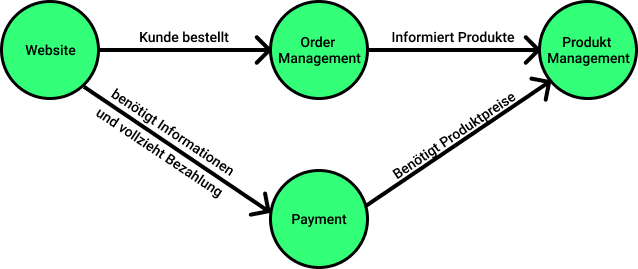
\includegraphics[width=1.0\linewidth]{img/prozess_eCommernce.png}
	\caption[Prozess Online-Shop]{Vereinfachter Prozess eines Online-Shops mit vier Komponenten\\ Quelle: Eigen}
	% \label{}
\end{figure}

% !TeX root = ../../master.tex
\section{Probleme und Herausforderungen im Bereich Gouvernance und Observability}

Viele Konzepte, welche für Microservices essenziell sind stellen mit einem strengen Blick auf die Gouvernance und die Observability eine Herausforderung dar. So werden im folgenden Teil einige dieser Konzepte vorgestellt und die damit verbundenen Probleme erläutert. Diese Probleme müssen mithilfe von Tooling oder eventuell sogar Designentscheidungen während der Softwareentwicklung verhindert werden.

\subsection{Design for Failure \autocite{FowlerMicrservices}}
Bei Design for Failure handelt es sich um ein Kernprinzip, welches bereits von \citeauthor{FowlerMicrservices} in seiner Zusammenstellung zu dem Arhcitekturprinzip Microservice in \enquote{\citetitle{FowlerMicrservices}} vorgestellt wurde. Die Idee hinter diesem Prinzip ist, dass Fehler immer, erst Recht im Softwareumfeld unvermeidbar sind. Deshalb müssen 


Design for Failure, aber wie bekomme ich es mit? Wie reagiere ich im Fehlerfall? Was muss getan werden, und wie groß sind die Auswirkungen wenn einer meiner tausend Microservices ausfällt? Diese und viele weitere Fragen müssen sich DevOps und Software-Engerneering Teams oftmals stellen, wenn sie sich in einer dezentralisierten Microservicearchitektur befinden. Es ist oftmals ein tiefes Verständnis des Zusammenspiels der einzelnen Services nötig um heruaszufinden, ob ein Fehler von eigenen Service kommt, oder ob es aufgrund eines Fehlers in einem anderen Service kommt. Das ultimative Ziel ist es dabei herauszufinden was das Problem ist und dieses auch schnellstmöglich zu beheben, sodass für den Endnutzer keine Merkbaren folgen auftreten. Microservices folgen dm Prinzip "Design for Failure", sodass eine Recovery möglich ist und ein operatives Business aufrecht erhalten werden kann. Trotz dieser hervorragenden Prämisse reicht ein \enquote{Design for Failure} alleine nicht aus. \enquote{Ein System ist nur so schlau wie das schwächste seiner Bestandteile}. Microservices mit dem Ziel kleiner dezentralisierter Services, welche einen spezialisiert sind auf eine bestimmte aufgabe innerhalb eines BusinessProzesses haben ironischerweise eine ihrer größten Schwäche in der Kommunikation miteinander. Es müssen Standards etabliert werden, sodass ServiceOwner einen wartbaren und funktionsfähigen Service entwickeln können. Es muss einen Software-Engeneer an einer Stelle ein Fehler unterlaufen und aufgrund der starken Kohäsion und Abhängigkeit der einzelnen Services unterneinander kann eine Reihe wichtiger Businessfunktionen davon betroffen sein. Im Beipsiel von Amazon führte ein Fehler in einem Service zu einer 20 Minütigen Downtime der Verkaufswebsite, was einem monetären Verlust von ca. 3.5 Mio Euro gleichkommt.

Kein Problem - \enquote{Design for Failure}. Ein Service fällt aus und ist darauf ausgelegt sich selbst wieder zu reaktivieren. Alle anderen Services können einen ausfall händeln. Soweit die Theorie. In der Praxis ist das leider nur allzuoft nicht der Fall. Innerhalb der Microservice-Gouvernance steht der Aspekt der dezentralisierten Entscheidungsfindung im Vordergrund. Das bedeutet, dass jedes Team das fachliche und unternehmerische Know-How zugesprochen wird das beste Tool und die beste Technologie für die von ihnen zu lösende Aufgabe zu wählen. Fängt ein Architekt nun an diese Aufgabe zu lösen, so benötigt er oftmals Informationen aus anderen Microservices, um seine Aufgabe zu erfüllen. 


\begin{center}
	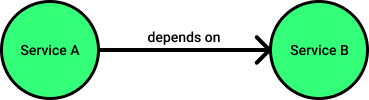
\includegraphics[width=0.55\linewidth]{img/service_dependency.png}
\end{center}

Es entsteht also eine Abhängigkeit zwischen zwei Microservices. Ebendieser angefragte Microservice benötigt aber wiederum einen anderen Service, um die angeforderte Information generieren zu können. Es entsteht also schon eine Kette von Abhängigkeiten. Was passiert, wenn ein Glied dieser Kette einen Fehler wirft? 

\Large Hier kommt ein Bild von einem Fehler in einer Microsericekette

\normalsize

Kein Problem - \enquote{Design for Failure}. Ein Architekt muss in der Planung seines Services die Möglichkeit haben, das Risiko und die Auswirkungen einen Ausfalls sowohl seines eigenen Services, als auch seiner Abhängigkeiten einschätzen zu können. Diese Einschätzung sollte auf Daten basieren, welche sowohl Information bisheriger Ausfälle und deren Ursachen enthalten als auch Ausblicke geben können auf den aktuellen Stand und eventuelle zukünftige Ausfälle.

Wie bereits Eingangs erwähnt ist bei der Betrachtung dieses Prinzips die Brille der Gouvernance und Observability aufgesetzt. Es ist ein wichtiger Bestandteil die Services innerhalb einer Unternehmensarchitektur so aufzubauen, dass diese trotz eins Fehlers ordnungsgemäß weiterlaufen und die Fähigkeit zur Recovery besitzen. Dieses Prinzip ist sogar dafür Veranwtortlich, dass Microservicepioniere wie Netflix innerhalb der Observability eine eigene, vierte Säule zu etablieren. Dabei handelt es sich um das sogenannte Chaos-Testing. Um dies kurz zu erläutern: Dabei handelt es sich um einen eigenen \enquote{Service}, welcher auf Basis von Chaos-Experimenten produktive Services ausschaltet und so die Recovery ebendieses Services und auch der davon abhängigen Services überprüfen kann. Dies bringt viele Vorteile mit sich und sorgt auch dafür, dass Services gut entwickelt sind. Diese Idee, wie das bewusste Einführen von Fehlern die generelle Qualität von Services verbessern kann, wird näher in \citetitle{AntifragileOrganization}\autocite{AntifragileOrganization} beschrieben.

\begin{itemize}
	\item Abgrenzung von Microservices gegenüber API's \\
	Wenn von Microservice Gouvernance und Observability geredet wird, ist oftmals die unterleigende Architektur mit Fokus auf VM-Daten usw gemeint. Wird von APIS gesprchen hat es oftmals mit business logik undso zutun
\end{itemize}
\begin{itemize}
	\item Welcher bereich soll observiert werden?
	\begin{itemize}
		\item Soll es um die hardware Daten (Memory, CPU, klassische cloud metriken) gehen oder um
		\item Softwareinformationen bzgl. software logging und tracing
	\end{itemize}
\end{itemize}


\section{Kriterien für gute Gouvernance}

Um im weiteren Verlauf der Arbeit die bereits bestehende und auch die vorgeschlagene Lösung zur Gouvernance und Observability von Microservice miteinander vergleichen zu können müssen einige Kriterien eingeführt werden. Um diese Kriterien zu erarbeiten wird auf vorherige Definition der Gouvernance und Observability geschaut \marginpar{Ref auf G \& O Def.}. Wie bereits zuvor festgestellt wurde besteht die Observability aus drei Säulen - dem \textit{Logging}, dem \textit{Tracing} und den \textit{Metriken}. Ein System welches zum Ziel hat Microservices zu observieren muss also auch in diesem drei Bereichen etwas beitragen. 

Des weiteren spielen Aspekte aus der Microservice Gouvernance eine Rolle für einene Technologie-Stack, welcher wie der hier vorgestellte versucht eine Brücke zwischen diesen beiden Bereichen zu bilden. Ein besonders großer und schwerwiegender Punkt der Microservice Gouvernance stellt eine dezentralisierte Verwaltung dar. Wie bereits \citeauthor{LeanixGouv} in seinem Artikel sagt:
\enquote{
	The main concept of these Microservices are the reusability of assets and tools which can be decentralized. The core theme of a decentralization governance is the concept of building and running it. This decentralized model is best suited for Microservices governances.
}\autocite{LeanixGouv}

Ein Tool welches in diesem Bereich helfen will, muss also als Entscheidungsstütze für dezentralisierte Serviecs funktionieren, um einen mehrwert zu schaffen. \\
Des weiteren muss eine Wertschöpfung aus den gewonnen Daten gezogen werden können. Es stellt also einen wichtigen Faktor dar, alle gesammelten Daten so aufzubereiten, dass es für den Nutzer dieses Tools einen Mehrwert bietet, welcher darüber hinausgeht nur einen Einblick in ebendiese Daten zu erhalten. Beispiele dafür wären Anwendungen im Bereich der \textbf{Predicitve Maintance} oder der \textbf{Anomaly Detection}, usw.

Tools, welche diesen Bereich abdecken müssen also in den folgenden drei großen Kriterien einen Mehrwert gegenüber bestehenden Lösungen bieten:

\begin{enumerate}
	\item Grundelgende Aspekte und Funktionen aus dem Bereich der Microservice Observability müssen abgedeckt sein. Dies beinhaltet die drei Säulen Logging, Tracing und Metriken.
	\item Die dezentralisierte Natur von Microservices muss gefördert werden, sodass ein Tool Entscheidungen - technischer oder unternehmerischer Natur - unterstützen und postiv beeinflussen kann.
	\item Gewonne Daten, egal aus welchen Bereich, müssen einen Mehrwert für den Nutzer darstellen, der über das reine Einsehen der gesammelten Daten hinausgeht.
\end{enumerate}

Auf Basis dieser drei Kriterien sollen nun bestehende Lösungen bewertet werden und mit der eigenen Lösungen verglichen werden, um festzustelle, ob die vorgeschlagene Lösungen
\begin{enumerate}
	\item den definiert Kriterien entspricht und
	\item einen nicht vorhandenen Mehrwert gegenüber bestehenden Lösungen bietet.
\end{enumerate}

Zuletzt ist es sehr wichtig, sollte ein neues Tool gewählt werden darauf zu achten, dass es offenen Standards folgt, um sicherzustelle, dass ein neues (oder bestehendes) System kompatibel ist und mit fremden Tools interagieren kann. Dies ist wichtig, damit auch Unternehmen sicherstellen können, dass der Aufwand, welcher mit der Einführung eines neuen Tolls kommt, ein lohnenswerter ist und eine langfristige Integration aufgrund von Kompatibilität als sinnvoll erachtet werden kann,

\section{Verschiedene Ansätze zum lösen von Gouvernance und Observability}
\subsection{Eigene Ansätze}
\subsection{Ansätze verschiedener Unternehmen}
\begin{itemize}
	\item Elastic \marginpar{Anomaly Detection}
	\item Neo4J \marginpar{ServiceRegistry (Idee für die Arbeit)}
	\item Netflix \marginpar{Master of Microservice}
\end{itemize}
Microservice Gouvernance und Themen der Observability sind bekannte Probleme und wurden schon oft von verschiedenen Organsiationen gelöst. Bewegt man sich im OpenSource bereich so findet sich mit der \ac{CNCF} ein Zusammenschluss, welcher versucht offene Standards für viele elementare Bereiche der Observability und der Gouvernance zu erreichen.

Die \ac{CNCF} definiert sich selbst folgendermaßen:

\enquote{
Cloud native Technologien ermöglichen es Unternehmen, skalierbare Anwendungen in modernen, dynamischen Umgebungen zu implementieren und zu betreiben. Dies können öffentliche, private und Hybrid-Clouds sein. Best-Practises, wie Container, Service-Meshs, Microservices, immutable Infrastruktur und deklarative APIs, unterstützen diesen Ansatz.

Die zugrundeliegenden Techniken ermöglichen die Umsetzung von entkoppelten Systemen, die belastbar, handhabbar und beobachtbar sind. Kombiniert mit einer robusten Automatisierung können Softwareentwickler mit geringem Aufwand flexibel und schnell auf Änderungen reagieren.

Die Cloud Native Computing Foundation fördert die Akzeptanz dieser Paradigmen durch die Ausgestaltung eines Open Source Ökosystems aus herstellerneutralen Projekten. Wir demokratisieren modernste und innovative Softwareentwicklungs-Patterns, um diese Innovationen für alle zugänglich zu machen.
}\autocite{CNCFGithub}

Die \ac{CNCF} vereint also mehrere Tools, welche allen offenen Standards folgen, damit Unternehmen unabhängig von großen Cloudanbietern wie \ac{GCP}, \ac{AWS} oder Microsoft Azure eine Cloud-Infrastruktur aufbauen können. Ein paar Beispiele der \ac{CNCF} zugehörigen Projekte sind treibende, grundlegende Softwarelösungen wie Kubernetes oder OpenShift.

Zusätzlich dient die \ac{CNCF} selbst auch als Organsiation, um verschiedene Industriestandards duchzusetzen. So wurde beispielsweise mithilfe der \textbf{Open Telemetry} ein Standard geschaffen, welcher Toolübergreifen das Sammeln und Auswerten verscheidener Tracingdaten ermöglicht. Dies ermöglicht einem Unternehmen, einen eigenen Stack zusammenzustellen, da es sich darauf verlassen kann, dass die Projekte, welche Teil der \ac{CNCF} sind miteinander kommunizieren und arbeiten können.

\url{https://landscape.cncf.io/category=coordination-service-discovery,service-proxy,service-mesh,observability-and-analysis&format=card-mode}

\section{Auf Basis der kriterien hergeleiteter eigener Ansatz mithilfe eines MicroserviceGraphen}

Innerhalb der Softwareentwicklung stellen sich die oben beschriebenen Probleme oftmals in ähnlicher Form dar. Ein praktisches Beispiel kommt aus dem Bereich der Webentiwcklung, in welchem Bundler ein ähnliches Problem zu bekämpfen haben. Diese besitzen zur Aufgabe Code, welcher in verschiedenen Dateien verteilt ist so zusammenzuführen, das später eine einzige syntaktisch korrete und ausführbare Datei vorliegt. Dabei muss allerdings bedacht werden, dass verschiedene Dateien unterschiedliche Codesegmente aus anderen Dateien importieren können und wiederum eigene Funktionen oder Variablen exportieren können. Dabei zählt es zu den Aufgaben eines Bundlers sicherzustellen, dass ein für die Programmiersprace valider Kontrollflow entsteht. Um dieses Problem zu lösen nutzen Bundler die Möglichkeit, einen Dependency-Graphen auf Basis der Imports und Exports aufzustellen. Dieser wird dann genutzt, um anhand des Startpunktes des Graphen die Zusammenführung der Dateien zu beginnen. Dabei müssen zusätzlich noch weitere Problem gelöst werden, da innerhaln eines Graphen auch circuläre Abhängigkeiten entstehen können, welche aufgelöst werden müssen. Ein Beispiel einer Zirkulären Abhängigkeit kann der \autoref{fig:GraphViz} entnommen werden.

\begin{itemize}
	\item Man es während CI/CD Stuff machen. Auch part von Microservices.
	\item Man kann es danach dynamisch nach Usage discovern lassen.
	\item Man kann einen kombinierten Ansatz wählen, um sowohl initial den Service inklusikve Metadaten sehen und danach die Nutzung ähnlich wie im Epsagon Dashboard zu sehen
\end{itemize}

\begin{figure}[h]
	\centering
	\makebox[\textwidth]{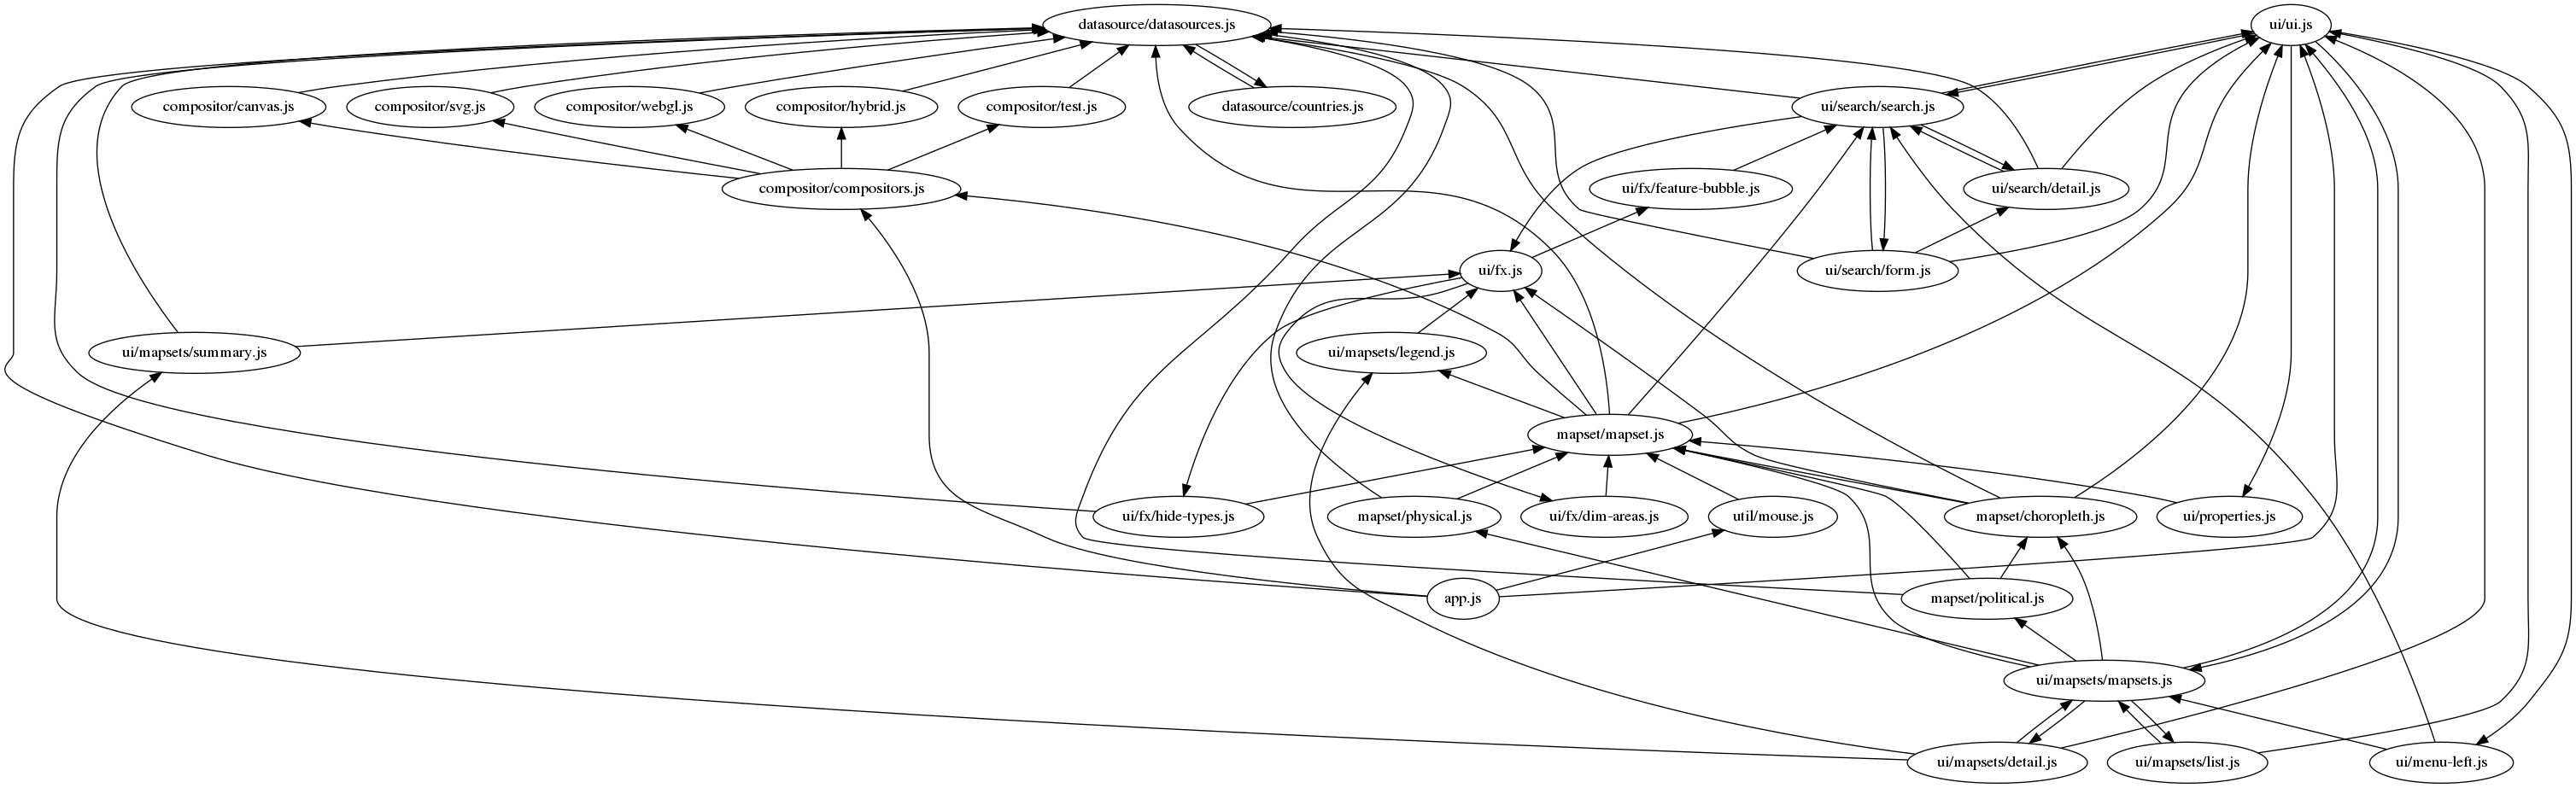
\includegraphics[width=\linewidth]{img/dependency-graph.png}}
	\caption[Dependency Graph]{Visulaisierung eines Dependency-Graphen mit zirkulären Abhängigkeiten. Quelle: \cite[]{GraphViz}}
	\label{fig:GraphViz}
\end{figure}
 All diese Elemente dienen als Grundlage zu der Idee, dass zur Risikoeinschätzung der Auswirkungen eines Fehelerfalls innerhalb einer Microservicearchitektur ein ähnlicher Dependency-Graph eine große Hilfe darstellen würde. Baut man den Graphen so auf, wie in obiger Analogie beschrieben, so erhält man einen Graphen, welcher Anzeigt ob und wie weit bestimmte Microservices miteinenander kommunizieren oder sogar voneinander Abhängigkeit sind. Dies beitet die Möglichkeit wertvolle Einblicke in das \textit{makroskopische} Zusammenspiel der einzelnen Komponenten einer Architektur zu erhalten. Ein Softwarearchitekt hat nun die Möglichkeit bei der Entscheidung über die Einführung eines neuen Service Informationen aus ebendiesem Graphen zu nutzen, um festzustellen ob eine zu Starke Abhängikteit zwischen Services vorhanden ist, oder ob es bei der Entwicklung bereits bestehende Abhängigkeiten gibt.
\marginpar{Hier eventuell bissjen über Kopplung auf Codebassis labern wie das Auswirkungen auf Arhcitektur haben kann} 
Der beschriebene Graph kann also als eine Art Service-Registry angesehen werden, welche Informationen zu der Beziehung zwischen verschiedenen Services beinhaltet. Gleichzeitig wird dadurch vor allem der Bereich der Microservice-Gouvernance betreten, wo eine Service-Registry eine zentrale Komponente darstellt. 

Zusammenfassend lässt sich das Konzept also folgendermaßen beschreiben: \\
Eine Schnittstelle zwischen Microservice-Gouvernance und -Observability wird mithilfe eines Dependency-Graphen gebildet. So spielen Aspekte einer Service-Registry und Elemente des Distributed-Tracing eine große Rolle in diesem Ansatz. 
\chapter{Idee und POC eines Microservice-Dependency Graphen}

Nun, da Grundlegende Begriffe geklärt wurden, werden Kriterien heruasgeabreitet, welche zur spätere Einschätzung und Bewertung eines vorgeschlagenen Ansatzes diesen sollen. Gleichzeitig werden diese Kriterien genutzt, um beretis bestehende Ansätze zu untersuchen und auf ihre Anwendbarkeit zu überprüfen.

Im Rahmen der Observability stehen drei große Säulen im Fokus:
\begin{enumerate}
	\item Logging
	\item Tracing
	\item Metriken
\end{enumerate}

Diese drei Elemente spielen eine wichtige Rolle um eine Lösung im Bereich der Observability liefern zu können. Im Rahmen dieser Arbeit wird vor allem ein Augenmerk auf den Status einer Microservice-Archtitektur gelegt, welche nicht zum Ziel hat, die softwaretechnische Ursache des Problems zu finden, sondern den Service oder den Container zu identifizieren, welcber für den Ausfall veranwtortlich ist. Gleichzeitig gibt es die Anforderung, dass die Abhängigkeiten verschiedener Microservices voneinander dargestellt und in Form von nutzbaren, auswertbaren Daten vorliegen. Hierbei kommt allerdings ein Punkt der Observability zu tragen, da dies, wie später näher erläutert wird auch mithilfe von Tracing erreicht werden kann.\\
Außerdem muss es möglich sein, die gewonnen Daten nutzbar zu machen, um nicht nur feststellen zu können, wecher Service die Ursache des Problems ist, sonder auch, um die Auswirkungen auf andere Services feststellen zu können. Es muss also ein einfacher Weg geschaffen werden, damit die Auswirkungen eines Fehlers schnell festgestellt werden können. 

\chapter{Bewertung und Einschätzung der Arbeit, sowie Ausbilck auf künfitge Arbeiten}
%	Literaturverzeichnis
\clearpage
\ihead{}
\printbibliography[title=Literaturverzeichnis]
\cleardoublepage

% Der Anhang beginnt hier - jedes Kapitel wird alphabetisch aufgezählt. (Anhang A, B usw.)
% \appendix
% \ihead{\appendixname~\thechapter} % Neue Header-Definition

% Ehrenwörtliche Erklärung ewerkl.tex einziehen
% !TEX root =  master.tex

\clearpage
\chapter*{Ehrenwörtliche Erklärung}

% Wird die folgende Zeile auskommentiert, erscheint die ehrenwörtliche
% Erklärung im Inhaltsverzeichnis.

% \addcontentsline{toc}{chapter}{Ehrenwörtliche Erklärung}
Ich versichere hiermit, dass ich die vorliegende Arbeit
 mit dem Thema: \textit{\DerTitelDerArbeit} selbstständig verfasst und keine anderen als die angegebenen Quellen und
Hilfsmittel benutzt habe. Ich versichere zudem,
dass die eingereichte elektronische Fassung mit der gedruckten Fassung übereinstimmt.

\vspace{3cm}
Mannheim, \today \hfill \DerAutorDerArbeit



\end{document}
